%\documentclass[12pt]{article}
%\usepackage[latin1]{inputenc}
%\usepackage[spanish]{babel}
%\usepackage{latexsym}
%\usepackage{amssymb}
%\usepackage{amsmath}

%\setlength{\textwidth}{15cm}

%\newtheorem{ejem}{Ejemplo}
%\newtheorem{teor}{Teorema}
%\begin{document}
\chapter{PRESENTACIÓN} % Write in your own chapter title
\label{Chapter1}
\lhead{Chapter 1. \emph{Chapter Title Here}} % Write in your own chapter title to set the page header

\section{INTRODUCCIÓN}
La dependencia causada por los sistemas informáticos en casi todas las actividades realizadas en los países, como ser la fabricación industrial, sistemas financieros, productos eléctricos, entre otros,
hacen que estos sistemas informáticos por la complejidad que presentan sean construidos a través de la ingeniería de software que comprenden de un conjunto de técnicas y herramientas que están en gran crecimiento debido a las exigencias, sin embargo mientras mas crezca nuestra capacidad de producir software, también lo hará la complejidad de los sistemas de software solicitados.\\

Es así como surgen diferentes herramientas para brindar apoyo dentro de las etapas de la ingeniera de software según cada metodología desempeñada. Una de las etapas que es imprescindible dentro de todas estas metodologías se encuentra el de implementación en el cual encontramos a una herramienta si bien no es obligatoria, resulta de gran ayuda e imprescindible hoy en día para la mayoría de las empresas y personas que se dedican a la elaboración de sistemas, hablamos de los sistemas de control de versiones que nos ayudan a la administración de las distintas versiones de cada producto desarrollado.\\

Encontramos una gran diversidad de sistemas de control de versiones, pero en este caso hacemos hincapié a uno de los mas populares como ser GIT, un sistema si bien no tan conocido como su adversario Subversion, pero que denota características ventajosas como ser la velocidad, reducción de tamaño,entre otras. es así como surge la idea de aportar una herramienta de apoyo para el desarrollo de software, como ser la comunicación de anuncios en tiempo real escritos por los integrantes del equipo de desarrollo como así también las acciones commit \footnote{commit (acción de cometer) se refiere a la idea de hacer que un conjunto de cambios "tentativos, o no permanentes" se conviertan en permanentes.} realizadas en cada uno de los repositorios locales que disponen, Publicadas a través de un sistema microblog.\\

pero ¿porque un microblog?, las actividades realizadas por cada integrante y las acciones en los repositorios son muy dinámicas por lo tanto sirven de gran ayuda el conocimiento del estado de cada uno de ellos, y lo hacemos mediante anuncios no muy largos publicados en el sistema de control de versiones, a través de forma automática gracias a la ayuda de algunos ganchos que nos brinda el sistema GIT y también a través del interprete de ordenes del sistema operativo, de esta manera se realizan las publicaciones de una manera menos perjuiciosa para el desarrollador, evitando perdidas de tiempo.\\

\section{PLANTEAMIENTO DEL PROBLEMA}

La comunicación entre los integrantes es esencial para el cumplimiento de los objetivos a alcanzar, para la coordinación eficaz del equipo de trabajo y la determinación de tiempos para las respectivas tareas asignadas.\\

La dificultad de tratar con cada uno de los integrantes de forma personal aumenta según el numero que estos integran y aun mas si realizan sus trabajos a distancia, esto causa mala comprensión de las tareas a cumplir dentro del desarrollo de software. Provocando perdidas de tiempo que en el transcurso son esenciales para la culminación del proyecto.\\

La mayoría de sistemas de control de versiones no se encuentran integrados a un sistema microblog, de ser así estos ayudarían a notificar que cambios acometidos que se están realizando en tiempo real a los ficheros de los repositorios de trabajo. Esta falta de comunicación provoca sincronización, causando conflictos a la hora de realizar actualizaciones en los repositorios.\\

GIT no es una excepción a estos posibles problemas, debido a que cada integrante del grupo de desarrollo obtiene una copia idéntica del repositorio y es responsable a mantenerlo en funcionamiento, es una de las cualidades de los sistemas de control de versiones distribuidas.\\

\section{OBJETIVOS}
\subsection{OBJETIVO GENERAL}
Desarrollar un sistema Web microblog\footnote{Microblog es un servicio que permite a sus usuarios enviar y publicar mensajes breves.
} para notificación de acciones aplicadas en repositorios locales de desarrollo de proyectos de software versionados con GIT\footnote{GIT software de sistema de control de versiones distribuido.\\
}.

\subsection{OBJETIVOS ESPECÍFICOS}
\begin{itemize}
\item Elegir herramientas que aporten al desarrollo del sistema
\item Analizar herramientas que faciliten la integración del sistema de control de versiones GIT con aplicaciones Web.
\item Realizar un asistente de configuración, para la comunicación de 	repositorios con el sistema Web(lado cliente).
\item Desarrollar el sistema web microblog, que permita registrar las acciones realizadas(commit) por los desarrolladores en los repositorios locales(lado servidor).
\end{itemize}

\section{JUSTIFICACIÓN}
El sistema web que se desea desarrollar ayudara  a los integrantes del grupo de trabajo encargados en la realización del proyecto, facilitando hacer un seguimiento de las tareas a realizar.\\

Los proyectos gestionados con el sistema de control de versiones GIT se podrán integrar con el sistema web microblog, debido a que se hará uso de algunos ganchos(hooks) que enlazarán con el sistema y así poder notificar a los integrantes del grupo de desarrollo en tiempo real sobre las acciones(commit) realizadas en cada uno de sus repositorios locales.\\

\section{METODOLOGÍA}
SCRUM es una metodología ágil, toma en cuenta la situación cambiante de los requisitos del cliente, así también minimiza la necesidad de la documentación.
Organizando el desarrollo de software de un manera evolutiva en los denominados sprints(periodos que duran de 15 a 30 días).

\subsection{PLANIFICACIÓN POR FASES}

\subsection{CALENDARIO DEL PROYECTO}

\subsubsection{ACTIVIDADES}
\begin{figure}[htb]
  Diagrama de Gantt
  \centering
  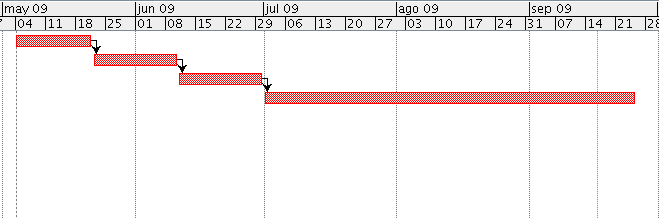
\includegraphics[width=0.9\textwidth]{imagenes/Gantt.png}%ext=pdf,jpg,png
  \caption{Diagrama de Gantt que muestra el tiempo de duración para el desarrollo del proyecto.}
  \label{contexto:figura}
\end{figure}

%\end{document}
